\documentclass[a4paper,12pt]{article}
\usepackage[utf8]{inputenc}
\usepackage[T1]{fontenc}
\usepackage[spanish]{babel}
\usepackage{csquotes}
\usepackage{anysize}
\usepackage{graphicx}
\marginsize{25mm}{25mm}{25mm}{25mm}

\title{{\scshape\bfseries Do Pigeons (}{\itshape\bfseries Columba livia}{\scshape\bfseries ) Use Information About the Absence of Food Appropriately? A Further look Into Suboptimal Choice}}
\author{\scshape\bfseries Inês Fortes, Armando Machado}
\date{2017}

\begin{document}
{\maketitle}

En ambientes inciertos, la información que da certidumbre de los resultados finales debería ser altamente valorada. Tanto que en algunas preparaciones los animales renuncian a reforzamiento primario para conseguir información, e.g., elección subóptima.

Según Vasconcelos, los mecanismos de decisión de los animales evolucionaron para optimizar la conducta en tareas naturales de forrajeo. En la naturaleza los organismos no deben pagar ningún costo de oportunidad al recibir malas noticias, así que los estímulos negativos y sus tiempos asociados son ignorados. En el laboratorio los obligamos a pagar ese costo quitándoles la oportunidad de usar la información, así que sus mecanismos resultan en malas elecciones. Aunque no pueden escapar, se `desinvolucran' del estímulo. Esta disparidad es lo que lleva a la elección subóptima. Basados en estas ideas, Vasconcelos y colaboradores desarrollaron el {\itshape Reinforcement Rate Model} (RRM).

{\scshape\bfseries The Reinforcement Rate Model}

Según la teoría de forrajeo óptimo la tasa de ingesta captura bien la adecuación a largo plazo de las estrategias de forrajeo, así que esta debería maximizarse. Suponiendo un escenario en el que un depredador encuentra la presa $i$ y la persigue, la atrapa con probabilidad $p_i$, y esta escapa con probabilidad $1-p_i$, la tasa de ingesta de la presa $i$ ($R_i$) está dada por
$$
R_i=\frac{p_i}{s+p_i\times (t+h) + (1-p_i)\times t}
$$
donde $s$ es el tiempo de búsqueda promedio, $p_i$ es la probabilidad de atrapar a la presa $i$, $t$ es el tiempo de persecución, y $h$ es el tiempo de manejo y consumo. En el laboratorio, $s$ sería el intervalo entre ensayos, $p_i$ la probabilidad de reforzamiento de una opción, $t$ la duración de los eslabones terminales, y $h$ la duración de reforzamiento. Según el análisis en el cual no se toman en cuenta los tiempos muertos, se debería retirar su influencia de la ecuación, y el ITI debería ser inconsecuente dado que ocurre después de la recompensa y porque es común a todas las consecuencias. Así, la tasa de recompensa para las alternativas informativa y no informativa estaría dada por
$$
R_{info}=\frac{p_{info}}{p_{info}\times (t+h)}=\frac 1{t+h}
$$
$$
R_{nonInfo}=\frac{p_{nonInfo}}{p_{nonInfo}\times(t+h)+(1-p_{nonInfo})\times t} = \frac{p_{nonInfo}}{t+p_{nonInfo}\times h} = \frac1{\frac{t}{0.5}+h}
$$
Así, $R_{info}$ siempre es mayor que $R_{nonInfo}$, con lo que se predice preferencia por la alternativa informativa. Dado que $1-p_{info}$ no se incluye en $R_{info}$ el modelo predice preferencia por la opción informativa sin importar la duración del estímulo negativo entanto su probabilidad de reforzamiento sea mayor que cero.

Se modificó al RRM para incluir la predicción clave de que, de poder, los animales usarán la información negativa y escaparán de los ensayos negativos.

{\scshape\bfseries The Prey Model and the RRM}

El prey model de Charnov predice que los animales deberían aceptar o rechazar una presa según qué elección lleve a la mayor tasa de recompensa a largo plazo. Pero esta maximización es distinta de la maximización del RRM: en el RRM la tasa de recompensa de cada opción es calculada de forma separada y los animales prefieren aquella con la tasa mayor. En el prey model las opciones no son informativa y no informativa, sino aceptar y rechazar, así que se enfoca la atención en la tasa promedio de ingesta bajo dos escenarios: uno en el que los animales siempre aceptan todos los estímulos (una estrategia generalista), y uno en el que rechazan al estímulo de malas noticias (estrategia especialista).

El modelo predice que la acción con la mayor tasa de recompensa siempre se implementa, porque las proporciones intermedias nunca maximizan la ingesta.

En el RRM original se asumía que los animales ignoran tanto el estímulo negativo como la duración del ITI, pero dado que ahora el interés está en la elección entre aceptar y rechazar, se asume que los animales deben poner atención a las consecuencias de cada curso de acción. Si un animal decide rechazar una alternativa en cuanto se presenta su TL, entonces el rechazo debería ser afectado solo por la duración del ITI (pero no la del TL, dado que éste fue evitado), y aceptar debería depender solo de la duración del TL (pero no del ITI). Es decir, solo las consecuencias inmediatas deberían afectar a la elección. Una estrategia generalista llevaría a una tasa de ingesta dada por
$$
R_{accept}=\frac{p_{reward}}{t+p_{reward}\times h}=\frac {1}{\frac{t}{p_{reward}} + h}
$$
donde $p_{reward}$ es la probabilidad de recompensa dada por el promedio ponderado de probabilidades de las opciones informativa y no-informativa.

Cuando los animales adoptan la estrategia especialista y rechazan el estímulo negativo solamente, las duraciones tomadas en cuenta dependen del estímulo presentado: si es el estímulo negativo, solo la duración del ITI ($s$)debe tomarse en cuenta; si se presenta el positivo, solo la duración del TL ($t$) se toma en cuenta. Así, la tasa de ingesta está dada por
$$
R_{reject}=\frac{p_{reward}}{t + p_{reward} \times h}=\frac{1}{\frac{t}{p_{reward}}+h}
$$
De estas ecuaciones se predice que los animales deberían escapar del estímulo negativo cuando 
$$
R_{reject} > R_{accept}
$$
$$
\frac{p_{reward}}{p_{bad-news}\times s + (1-p_{bad-news}) \times t + p_{reward}\times h}>\frac{1}{\frac{t}{p_{reward}}+h}
$$
que se simplifica a
$$ s <t $$
es decir, que los animales deberían escapar del estímulo negativo si la duración del ITI es menor que la duración del TL, pues entonces ocurre el punto de inflexión en el que la tasa de reforzamiento de la estrategia generalista pasa a ser menor que la tasa de la estrategia especialista. Ni la probabilidad de reforzamiento ni su duración influyen en la decisión de escapar.

{\scshape\bfseries The Present Experiments}

La meta de estos experimentos es probar la hipótesis del RRM: los animales deberían escapar en presencia del estímulo negativo. Una segunda meta es determinar la influencia que tiene la duración de TL y ITI en las respuestas de escape. Aunque solo las estrategias absolutas pueden ser óptimas, se ha mostrado que la probabilidad de escapar suele ser intermedia. Se anticipa que acortar el ITI debería llevar a más respuestas de escape comparadas con alargar la duración del TL.

Finalmente, la función de esta investigación también es semántica: se busca aclarar qué quieren decir los investigadores cuando dicen que el estímulo negativo es ignorado: si ignorar el estímulo negativo significa que el animal está subjetivamente en una situación en la cual no hay estímulo negativo, entonces jamás escaparía. Si ignorarlo significa que, aunque el animal está consciente de su presencia, simplemente se desinvolucra de la tarea y no asocia la presentación del estímulo con la elección de la alternativa informativa (un problema de atribución de crédito), entonces debería escapar porque al hacerlo disminuye la demora hacia la siguiente posible recompensa. El RRM presupone lo segundo.

{\scshape\bfseries Experimento I - El efecto de la duración del ITI en la conducta de escape}

Usaron el procedimiento de elección subóptima con TL de TF10s. El ITI fue de 10s también. Sin embargo, cuando se presentaba cualquiera de los TL, los animales podían escapar de él picando la tecla central, lo que terminaba el ensayo inmediatamente y comenzaba el ITI.

{\bfseries Ensayos de escape forzado.} Dado que las respuestas de escape tendieron a disminuir, se intodujeron ensayos de escape forzado en los cuales se apagaban todas las teclas salvo por la tecla central. Responder en ella iniciaba el ITI. Estos ensayos se distribuyeron entre los ensayos normales para garantizar que las palomas tenían contacto consistente con sus contingencias.

{\bfseries ITI de 1 segundo.} Todos los ITI se redujeron a 1s.

{\bfseries Escape de los eslabones iniciales.} Los animales no deberían escapar en los IL dado que no proveen información sobre la comida inminente. Para probarlo, se agregó la posibilidad de escapar de los IL y se agregaron ensayos de escape forzado a los IL. Escapar de los IL tenía como resultado pasar al ITI de 1s inmediatamente.

{\bfseries Resultados y discusión}

Inicialmente se observó una tendencia para escoger la alternativa óptima. La preferencia rápidamente se revirtió y se mantuvo durante las fases siguientes.

{\bfseries Respuestas de escape.} Los escapes ocurrieron casi exclusivamente en presencia del estímulo negativo. Los escapes incrementaron con la fase de escapes forzados.

Los escapes estuvieron por debajo del 50\% esperado (dado que la tasa de reforzamiento esperada es la misma si se escapa o no se escapa), lo que inidicó la presencia de un sesgo en contra de escapar, debido probablemente a que el escape tiene un mayor requisito de respuesta que el no-escape (consistente con resultados de Lea (1979) y Mazur (2007)).

En las últimas dos fases con ITI de 1s (y por lo tanto mayor tasa de reforzamiento por rechazar que por aceptar) el escape incrementó cosiderablemente.

En la última fase las palomas rara vez escaparon del IL.

En resumen, se confirmaron las predicciones del RRM. Las palomas escaparon solo del estímulo de malas noticias, escaparon más cuando la tasa de recompensa por escapar era mayor que la recompensa por aceptar, y casi nunca escaparon en los ILs.

{\scshape\bfseries Experimento 2 -  El efecto de la duración del TL en la conducta de escape}

Obervaciones informales mostraron que cuando se presentaba el estímulo negativo, las palomas le daban la espalda, lo que pudo contribuir a su sesgo contra escapar. En el experimento 2 se cambió la posición de la tecla de escape. Esto además permitió que la respuesta natural de la paloma ante el $S^-$ coocurriera con la operante de escape. También se manipuló la duración de los TL manteniendo el ITI constante. Se esperaba que incrementaran las respuestas de escape conforme aumentaba la duración del TL.

Dado que se utilizó una nueva caja operante alargada para separar la respuesta de escape del estímulo negativo, se probó inicialmente elección subóptima estándar antes de introducir respuestas de escape. Tras ello, se introdujo la operante de escape con sus ensayos forzados correspondientes. Los ITI y los TL eran de 10 segundos.

\begin{figure}[ht]
	\begin{center}
		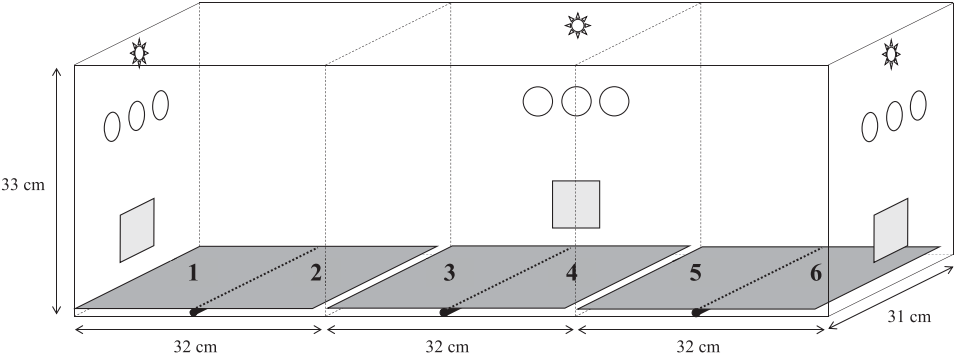
\includegraphics[scale=0.5]{Fortes.png}
	\end{center}
\end{figure}	

{\bfseries Escape de TLs de 20s.} Se incrementó la duración de los TL de 10 a 20s. 

{\bfseries Resultados y discusión}

Todas las aves prefirieron la alternativa informativa.

{\bfseries Respuestas de escape.} Solo escaparon del estímulo negativo. En la primera fase el escape se mantuvo aun debajo de 50\%. Cuando en el primer experimento, con la operante de escape cerca al estímulo negativo, se encontró una proporción de escapes de 26\%, en el segundo experimento con distancias incrementadas se encontró una proporción de escapes de 10\%, lo que indica que la evitación del estímulo negativo no explica el sesgo en contra del escape, y éste se debió probablemente a la diferencia en requisitos de respuesta.

Cuando la duración del TL se incrementó de 10 a 20s (haciendo que la tasa de recompena por rechazar fuese más grande que la tasa por aceptar) la proporción de escapes incrementó a 53\%, lo que es consistente con el RRM.

{\bfseries Movimiento.} Se registró la posición de las palomas durante las sesiones. El análisis mostró que en elección subóptima estándar, las aves permanecieron cerca de la tecla escogida excepto cuando se presentaba el estímulo  negativo, en cuyo caso se movían al centro de la caja hasta el siguiente ensayo.

Este alejamiento podría ser el resultado de la aversión generada por el estímulo negativo, o de la disponibilidad de más tiempo para moverse.

Se confirma la observación informal de que los animales se alejan del estímulo negativo. Las palomas se alejaban de él incluso en los ensayos en los cuales no escapaban.

¿Por qué se movían a la tecla de escape en la mayoría de los ensayos, pero solo escapaban en algunos? Quizá las dos conductas están controladas por variables diferentes. Quizá alejarse es una respuesta incondicionada ante los estímulos negativos para maximizar la probabilidad de encontrar comida, mientras que el escape podría ser una operante mantenida por sus consecuencias(por ello solo escapaban cuando era ventajoso hacerlo).

{\scshape\bfseries General Discussion}

La explicación más consistente para elección subóptima es que los animales toman en cuenta los estímulos positivos en ambas alternativas pero ignoran el estímulo negativo, lo que lleva a una tasa percibida más alta para la alternativa informativa.

Según Vasconcelos, la elección subóptima resulta al evaluar a los animales en una situación en la cual la información es inútil, cuando los organismos evolucionaron en situaciones en las cuales la información es funcional. En este experimento se hizo útil a la información. Se predijo, según el RRM, que (1) los animales escaparían solamente del estímulo negativo, (2) que el escape incrementaría según la tasa de recompensa derivada de escapar incrementa con respecto a aceptar, como al reducir el ITI o al aumentar el TL, y (3) que la probabilidad de escapar debería estar asociada con el grado de mejoría en la tasa de recompensa cuando se rechaza el estímulo de malas noticias comparada con cuando éste se acepta.

Las predicciones 1 y 2 fueron confirmadas por ambos experimentos.

El modelo predice mayor tasa de escape cuando el ITI es más corto que el TL, lo cual sucedió (ITI = 1s, TL = 10s). Sin embargo se puede argumentar que las palomas escaparon más en esa situación debido a dos razones: en el experimento 1 la reducción en demora a la comida era más notable cuando ITI = 1 que cuando ITI = 10. En el experimento 2 pudo haber más escapes cuando TL = 20 simplemente porque ello da más oportunidades para escapar. Estas posibilidades permanecen abiertas.

Mientras, se identifican dos problemas con esas interpretaciones: si las palomas están siendo sensibles a la reducción de la demora en el experimento 1, ¿por qué no revertir su preferencia y así reducir aun más la demora a la siguiente entrega de comida? ¿Los animales escaparían si no hubiese reducción en la demora, sino que la única función del escape fuera la terminación del estímulo negativo? Segundo, si las palomas escaparon más en el experimento dos porque tenían más tiempo para hacerlo, el número de escapes dentro de los primeros 10s del TL debería ser el mismo en ambas condiciones, pero los datos fueron ambiguos a ese respecto.

Para probar la última predicción se comparó la proporción de escapes con el incremento en recompensa derivado de escapar del estímulo negativo. La comparación mostró que los animales escaparon en mayor proporción cuando escapar era más redituable. Sin embargo, las predicciones del RRM son solo aproximaciones a lo que se espera que los animales hagan, dado que (1) no se consideran las latencias de respuesta, (2) se asume que todos los ITI tienen efectos similares sobre la tasa de recompensa percibida (aunque hay evidencia que pone eso en duda), y (3) se predice un patrón de escape de todo o nada aunque lo observado es una proporción intermedia.

Las latencias de escape al estímulo negativo deberían agregarse al $s$ del denominador del modelo, lo que reduciría $R_{reject}$. Los datos indican que la latencia debería excluirse del análisis, pero el problema es meritorio de más investigación.

El hecho de que los animales escaparon del estímulo negativo indica que el estímulo no se ignoraba en el sentido de que los animales estuviesen subjetivamente en una situación sin él. La preferencia por la alternativa informativa sugiere que quizá los animales no le atribuyen el estímulo negativo a esa alternativa. Esto en conjunto indica que el estímulo es ignorado en el sentido de que los animales no lo asocian con la alternativa informativa. Esto explica por qué incrementar su duración a 200s no tuvo ningún efecto en la preferencia (Fortes, 2016).

En conclusión, se adaptó una tarea de elección para hacerla más similar a una situación natural de forrajeo, haciendo útil a la información. Los resultados se ajustan al RRM. Los experimentos además muestran que los animales sí le prestan atención al estímulo negativo, pues se alejan y escapan de él, pero el estímulo no se asocia con la alternativa informativa.

\end{document}
